% This LaTeX was auto-generated from MATLAB code.
% To make changes, update the MATLAB code and export to LaTeX again.

\documentclass{article}

\usepackage[utf8]{inputenc}
\usepackage[T1]{fontenc}
\usepackage{lmodern}
\usepackage{graphicx}
\usepackage{color}
\usepackage{hyperref}
\usepackage{amsmath}
\usepackage{amsfonts}
\usepackage{epstopdf}
\usepackage[table]{xcolor}
\usepackage{matlab}
\usepackage[paperheight=795pt,paperwidth=614pt,top=72pt,bottom=72pt,right=72pt,left=72pt,heightrounded]{geometry}

\sloppy
\epstopdfsetup{outdir=./}
\graphicspath{ {./2024-03-01-matlab-regression_media/} }

\matlabhastoc

\begin{document}

\label{T_C685BDF0}
\matlabtitle{MATLAB basics and regression}

\matlabtableofcontents{Table of Contents}
\label{H_2EBE8B68}
\matlabheading{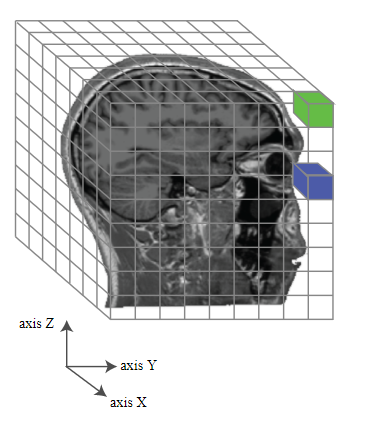
\includegraphics[width=\maxwidth{20.873055694932262em}]{image_0}}

\label{H_1A80E756}
\matlabheading{0. Why MATLAB?}

\begin{par}
\begin{flushleft}
MATLAB is a proprietary programming language and computing enviorment developed by MathWorks. It is specifically desinged for engineers and scientists who work with data matrices of large sizes. Some of its advantages over other options (e.g., R, Python) include:
\end{flushleft}
\end{par}

\begin{itemize}
\setlength{\itemsep}{-1ex}
   \item{\begin{flushleft} having a graphical user interface (GUI) \end{flushleft}}
   \item{\begin{flushleft} (relatively) easy-to-understand data types \end{flushleft}}
   \item{\begin{flushleft} comprehensive tried-and-tested built-in functions \end{flushleft}}
   \item{\begin{flushleft} various toolboxes for brain research and beyond \end{flushleft}}
\end{itemize}

\begin{par}
\begin{flushleft}
Here are some famous/useful fMRI packages that you might use:
\end{flushleft}
\end{par}

\begin{tabular} {|p{50pt}|p{382.2285461425781pt}|}\hline
\begin{par}
\begin{flushleft}
\href{https://www.fil.ion.ucl.ac.uk/spm/software/spm12/}{SPM}
\end{flushleft}
\end{par}

 & \begin{par}
\begin{flushleft}
one of the most popular packages for preprocessing and analyzing neuroimaging data, besides FSL and AFNI
\end{flushleft}
\end{par}

\\
\hline
\begin{par}
\begin{flushleft}
\href{https://web.conn-toolbox.org/}{CONN}
\end{flushleft}
\end{par}

 & \begin{par}
\begin{flushleft}
MATLAB- and SPM-based interactive toolbox for analyzing brain connectivity 
\end{flushleft}
\end{par}

\\
\hline
\begin{par}
\begin{flushleft}
\href{https://sccn.ucsd.edu/eeglab/index.php}{EEGLAB}
\end{flushleft}
\end{par}

 & \begin{par}
\begin{flushleft}
interactive toolbox for processing EEG, MEG, and other electrophysiological data
\end{flushleft}
\end{par}

\\
\hline
\begin{par}
\begin{flushleft}
\href{https://www.fieldtriptoolbox.org/}{FieldTrip}
\end{flushleft}
\end{par}

 & \begin{par}
\begin{flushleft}
non-interactive toolbox for processing MEG, EEG, and iEEG data
\end{flushleft}
\end{par}

\\
\hline
\begin{par}
\begin{flushleft}
\href{http://psychtoolbox.org/}{PsychToolbox}
\end{flushleft}
\end{par}

 & \begin{par}
\begin{flushleft}
toolbox for controling visual and auditory stimulus presentation 
\end{flushleft}
\end{par}

\\
\hline
\end{tabular}


\vspace{1em}
\begin{par}
\begin{flushleft}
And here are some previous DIBS Methods Meeting posts that used MATLAB to some extent: 
\end{flushleft}
\end{par}

\begin{itemize}
\setlength{\itemsep}{-1ex}
   \item{\begin{flushleft} \href{https://dibsmethodsmeetings.github.io/matlab-basics/}{MATLAB basics} \end{flushleft}}
   \item{\begin{flushleft} \href{https://dibsmethodsmeetings.github.io/multivariate-pattern-analysis/}{Multivariate pattern analysis} \end{flushleft}}
   \item{\begin{flushleft} \href{https://dibsmethodsmeetings.github.io/eeg-analysis/}{EEG Preprocessing using EEGLAB}  \end{flushleft}}
   \item{\begin{flushleft} \href{https://dibsmethodsmeetings.github.io/fourier-transforms/}{Decomposing Fourier transforms} \end{flushleft}}
\end{itemize}

\label{H_4D61C4EC}
\matlabheading{1. Getting started}

\begin{par}
\begin{flushleft}
Let's get started! If you haven't installed MATLAB or want to familiarize yourself with the GUI, please refer to \href{https://dibsmethodsmeetings.github.io/matlab-basics/}{my earlier post on MATLAB basics} OR try out the online version here: \href{https://matlab.mathworks.com}{https://matlab.mathworks.com/.}
\end{flushleft}
\end{par}


\label{H_C69F7016}
\matlabheading{2. Data types and operations}

\begin{par}
\begin{flushleft}
This was covered in a bit more depths in \href{https://dibsmethodsmeetings.github.io/matlab-basics/}{my earlier post}, but I thought I would do a quick review of some important things here because they are going to come up later as we talk about regression.
\end{flushleft}
\end{par}

\label{H_95785FA9}
\matlabheadingthree{Numeric types}

\begin{par}
\hfill \break
\end{par}

\begin{matlabcode}
% double	Double-precision arrays (64-bit) <-- MATLAB default
% single	Single-precision arrays (32-bit)
% int8	    8-bit signed integer arrays
% uint8	    8-bit unsigned integer arrays
% ...
% for example:
class(1) % use the function class to check data types
\end{matlabcode}
\begin{matlaboutput}
ans = 'double'
\end{matlaboutput}
\begin{matlabcode}
% use space or comma to separate columns
% use semicolon to separate rows
% use square brackets [ ] to put things together
a = [1    2,    NaN;
    .5    Inf   nan] % this is a 2 x 3 double array
\end{matlabcode}
\begin{matlaboutput}
a = 2x3    
    1.0000    2.0000       NaN
    0.5000       Inf       NaN

\end{matlaboutput}
\begin{matlabcode}
% note the two special numbers: Inf and NaN (not a number)
class(a) % the data type is still 'double'
\end{matlabcode}
\begin{matlaboutput}
ans = 'double'
\end{matlaboutput}

\label{H_D5A335BB}
\matlabheadingthree{Characters and Strings}

\begin{par}
\hfill \break
\end{par}

\begin{matlabcode}
% use single quotes for characters
char1 = 'a';
char2 = 'abc';
% use double quotes for strings
str1 = "a";
str2 = "abc";
% check data types
class(char1);
class(str1);
% difference
length(char2)
\end{matlabcode}
\begin{matlaboutput}
ans = 3
\end{matlaboutput}
\begin{matlabcode}
length(str2)
\end{matlabcode}
\begin{matlaboutput}
ans = 1
\end{matlaboutput}
\begin{matlabcode}
% if we want to concatnate different things
[char1 char2] % correctly concatenated character array
\end{matlabcode}
\begin{matlaboutput}
ans = 'aabc'
\end{matlaboutput}
\begin{matlabcode}
str1 + str2 % correctly concatenated strings
\end{matlabcode}
\begin{matlaboutput}
ans = "aabc"
\end{matlaboutput}
\begin{matlabcode}
char1 + char2 % data type converted to numeric for addition
\end{matlabcode}
\begin{matlaboutput}
ans = 1x3    
   194   195   196

\end{matlaboutput}
\begin{matlabcode}
[char1 str2] % character coerced to string
\end{matlabcode}
\begin{matlaboutput}
ans = 1x2 string    
"a"          "abc"        

\end{matlaboutput}

\label{H_6FBC0609}
\matlabheadingthree{Tables}

\begin{par}
\hfill \break
\end{par}

\begin{matlabcode}
T = table;
T.col1 = [1; 2];
T.col2 = ["hello"; "world"];
T
\end{matlabcode}
\begin{matlabtableoutput}
{
\begin{tabular} {|c|c|c|}\hline
\mlcell{ } & \mlcell{col1} & \mlcell{col2} \\ \hline
\mlcell{1} & \mlcell{1} & \mlcell{"hello"} \\ \hline
\mlcell{2} & \mlcell{2} & \mlcell{"world"} \\ 
\hline
\end{tabular}
}
\end{matlabtableoutput}
\begin{matlabcode}
% dimensions must match
T.col3 = repmat(3, height(T), 1);
try T.col4 = 4; catch err; disp(err); end
\end{matlabcode}
\begin{matlaboutput}
  MException with properties:

    identifier: 'MATLAB:table:RowDimensionMismatch'
       message: 'To assign to or create a variable in a table, the number of rows must match the height of the table.'
         cause: {}
         stack: [2x1 struct]
    Correction: []
\end{matlaboutput}
\begin{matlabcode}
% data type must be consistent within each row
T.col2(2) = 1;
T % see how 1 is coerced into "1"
\end{matlabcode}
\begin{matlabtableoutput}
{
\begin{tabular} {|c|c|c|c|}\hline
\mlcell{ } & \mlcell{col1} & \mlcell{col2} & \mlcell{col3} \\ \hline
\mlcell{1} & \mlcell{1} & \mlcell{"hello"} & \mlcell{3} \\ \hline
\mlcell{2} & \mlcell{2} & \mlcell{"1"} & \mlcell{3} \\ 
\hline
\end{tabular}
}
\end{matlabtableoutput}
\begin{matlabcode}
class(T.col2)
\end{matlabcode}
\begin{matlaboutput}
ans = 'string'
\end{matlaboutput}

\label{H_2D6BE0C5}
\matlabheadingthree{Cell Arrays}

\begin{par}
\hfill \break
\end{par}

\begin{matlabcode}
% use curly brackets to put together things of different sizes and types
C = {42, "abcd"; table(nan), [1 2 3]; Inf, {}}
\end{matlabcode}
\begin{matlabtableoutput}
{
\begin{tabular} {|c|c|c|}\hline
\mlcell{ } & \mlcell{1} & \mlcell{2} \\ \hline
\mlcell{1} & \mlcell{42} & \mlcell{"abcd"} \\ \hline
\mlcell{2} & \mlcell{1x1 table} & \mlcell{[1,2,3]} \\ \hline
\mlcell{3} & \mlcell{Inf} & \mlcell{0x0 cell} \\ 
\hline
\end{tabular}
}
\end{matlabtableoutput}
\begin{matlabcode}
C(2) % paratheses indexing retrieves the cell 
\end{matlabcode}
\begin{matlaboutput}
ans = 
    {1x1 table}

\end{matlaboutput}
\begin{matlabcode}
C{2} % curly braces indexing retrieves the cell *content*
\end{matlabcode}
\begin{matlabtableoutput}
{
\begin{tabular} {|c|c|}\hline
\mlcell{ } & \mlcell{Var1} \\ \hline
\mlcell{1} & \mlcell{NaN} \\ 
\hline
\end{tabular}
}
\end{matlabtableoutput}

\begin{par}
\begin{flushleft}
Arrays are effcient, but make sure you access the in the correct order.
\end{flushleft}
\end{par}

\begin{matlabcode}
% double arrays are indexed with parentheses
a = [11 12 13; 21 23 24]; % 2 x 3 double array
a
\end{matlabcode}
\begin{matlaboutput}
a = 2x3    
    11    12    13
    21    23    24

\end{matlaboutput}
\begin{matlabcode}
a(1, 2) % row 1, column 2
\end{matlabcode}
\begin{matlaboutput}
ans = 12
\end{matlaboutput}
\begin{matlabcode}
a(1:end, 2) % all rows, column 2
\end{matlabcode}
\begin{matlaboutput}
ans = 2x1    
    12
    23

\end{matlaboutput}
\begin{matlabcode}
a(2, :) % row 2, all columns
\end{matlabcode}
\begin{matlaboutput}
ans = 1x3    
    21    23    24

\end{matlaboutput}
\begin{matlabcode}
% here's something that may seem odd
a(4) % 4th entry
\end{matlabcode}
\begin{matlaboutput}
ans = 23
\end{matlaboutput}
\begin{matlabcode}
a(:) % all entries
\end{matlabcode}
\begin{matlaboutput}
ans = 6x1    
    11
    21
    12
    23
    13
    24

\end{matlaboutput}

\begin{par}
\begin{flushleft}
In Python and R, array data is stored \textbf{row-wise}. In contrast, MATLAB arrays are stored \textbf{column-wise}, even though they are easily defined row-wise. 
\end{flushleft}
\end{par}

\begin{par}
\begin{flushleft}
┑( ̄Д  ̄)┍ 
\end{flushleft}
\end{par}

\label{H_236DB427}
\matlabheadingthree{Structures}

\begin{par}
\hfill \break
\end{par}

\begin{matlabcode}
% group data using fields
% each field can be of any data type, including structures
S = struct;
S.field1_struct = struct;
S.field2_cell = C;
S.field3_table = T;
S.field4_char = char1;
S
\end{matlabcode}
\begin{matlaboutput}
S = 
    field1_struct: [1x1 struct]
      field2_cell: {3x2 cell}
     field3_table: [2x3 table]
      field4_char: 'a'

\end{matlaboutput}


\label{H_006DC13C}
\matlabheading{3. Regression}

\begin{par}
\begin{flushleft}
Let's talk about regression! Through the official \href{https://www.mathworks.com/products/statistics.html}{Statistics and Machine Learning Toolbox}, we have access to several built-in MATLAB functions for regression. 
\end{flushleft}
\end{par}

\begin{par}
\begin{flushleft}
First, let's load some data. We are going to use an \href{https://www.kaggle.com/datasets/kumarajarshi/life-expectancy-who}{open dataset on Kaggle on life expectancy}. The original data came from the World Health Organization (WHO), who has been keeping track of the life expectancy and many other health factors of all countries. The final dataset consists of 20 predictor variables and 2938 rows, containing information for 193 countries between 2000 and 2015.
\end{flushleft}
\end{par}

\begin{matlabcode}
data_table = readtable("2024-03-01-matlab-regression-Life-Expectancy.csv", ...
    "VariableNamingRule", "preserve"); % preserve white space in column names for readability
head(data_table);
\end{matlabcode}
\begin{matlaboutput}
        Country        Year        Status        Life expectancy    Adult Mortality    infant deaths    Alcohol    percentage expenditure    Hepatitis B    Measles    BMI     under-five deaths    Polio    Total expenditure    Diphtheria    HIV/AIDS     GDP      Population    thinness  1-19 years    thinness 5-9 years    Income composition of resources    Schooling
    _______________    ____    ______________    _______________    _______________    _____________    _______    ______________________    ___________    _______    ____    _________________    _____    _________________    __________    ________    ______    __________    ____________________    __________________    _______________________________    _________

    {'Afghanistan'}    2015    {'Developing'}           65                263               62           0.01               71.28                65          1154      19.1            83             6            8.16               65          0.1       584.26    3.3736e+07            17.2                   17.3                        0.479                   10.1   
    {'Afghanistan'}    2014    {'Developing'}         59.9                271               64           0.01              73.524                62           492      18.6            86            58            8.18               62          0.1        612.7    3.2758e+05            17.5                   17.5                        0.476                     10   
    {'Afghanistan'}    2013    {'Developing'}         59.9                268               66           0.01              73.219                64           430      18.1            89            62            8.13               64          0.1       631.74    3.1732e+07            17.7                   17.7                         0.47                    9.9   
    {'Afghanistan'}    2012    {'Developing'}         59.5                272               69           0.01              78.184                67          2787      17.6            93            67            8.52               67          0.1       669.96     3.697e+06            17.9                     18                        0.463                    9.8   
    {'Afghanistan'}    2011    {'Developing'}         59.2                275               71           0.01              7.0971                68          3013      17.2            97            68            7.87               68          0.1       63.537    2.9786e+06            18.2                   18.2                        0.454                    9.5   
    {'Afghanistan'}    2010    {'Developing'}         58.8                279               74           0.01              79.679                66          1989      16.7           102            66             9.2               66          0.1       553.33    2.8832e+06            18.4                   18.4                        0.448                    9.2   
    {'Afghanistan'}    2009    {'Developing'}         58.6                281               77           0.01              56.762                63          2861      16.2           106            63            9.42               63          0.1       445.89    2.8433e+05            18.6                   18.7                        0.434                    8.9   
    {'Afghanistan'}    2008    {'Developing'}         58.1                287               80           0.03              25.874                64          1599      15.7           110            64            8.33               64          0.1       373.36    2.7294e+06            18.8                   18.9                        0.433                    8.7   
\end{matlaboutput}

\begin{par}
\begin{flushleft}
Let's validate the information in the description above.
\end{flushleft}
\end{par}

\begin{matlabcode}
fprintf( ...
    "Number of rows = %d \n" + ...
    "Number of years = %d \n" + ...
    "Number of countries = %d \n", ...
    height(data_table), ...
    length(unique(data_table.Year)), ...
    length(unique(data_table.Country)));
\end{matlabcode}
\begin{matlaboutput}
Number of rows = 2938 
Number of years = 16 
Number of countries = 193 
\end{matlaboutput}

\begin{par}
\begin{flushleft}
For simplicity, we are going to focus on the most recent complete sample (year 2014) and on the following variables:
\end{flushleft}
\end{par}

\begin{itemize}
\setlength{\itemsep}{-1ex}
   \item{\begin{flushleft} Life expectancy (in years) \end{flushleft}}
   \item{\begin{flushleft} Status: "Developed", "Developing" \end{flushleft}}
   \item{\begin{flushleft} Total expenditure: General government expenditure on health as a percentage of total government expenditure (\%) \end{flushleft}}
\end{itemize}

\begin{matlabcode}
data_2014 = data_table(data_table.Year==2014, ["Country" "Status" "Total expenditure" "Life expectancy"]);
head(data_2014);
\end{matlabcode}
\begin{matlaboutput}
            Country                Status        Total expenditure    Life expectancy
    _______________________    ______________    _________________    _______________

    {'Afghanistan'        }    {'Developing'}          8.18                59.9      
    {'Albania'            }    {'Developing'}          5.88                77.5      
    {'Algeria'            }    {'Developing'}          7.21                75.4      
    {'Angola'             }    {'Developing'}          3.31                51.7      
    {'Antigua and Barbuda'}    {'Developing'}          5.54                76.2      
    {'Argentina'          }    {'Developing'}          4.79                76.2      
    {'Armenia'            }    {'Developing'}          4.48                74.6      
    {'Australia'          }    {'Developed' }          9.42                82.7      
\end{matlaboutput}

\begin{par}
\begin{flushleft}
Before actually fitting a linear regression model, let's plot the data.
\end{flushleft}
\end{par}

\begin{matlabcode}
close all
figure
gscatter( ...
    data_2014.("Total expenditure"), ... x-axis
    data_2014.("Life expectancy"), ... y-axis
    data_2014.Status ... color
    );
title("Life Expectancy against Healthcare Expenditure in 2014")
\end{matlabcode}
\begin{center}
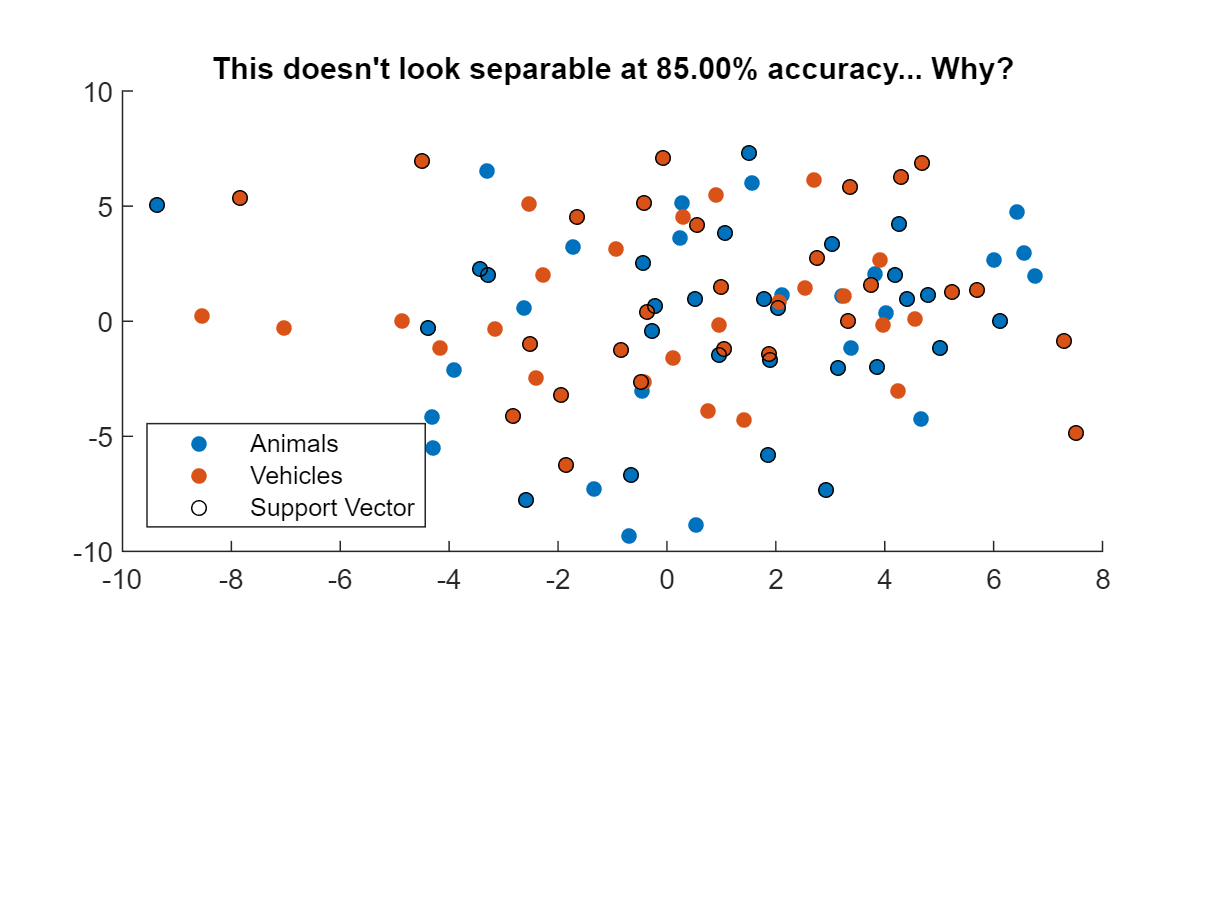
\includegraphics[width=\maxwidth{56.196688409433015em}]{figure_0.eps}
\end{center}

\begin{par}
\begin{flushleft}
We make 3 observations:
\end{flushleft}
\end{par}

\begin{enumerate}
\setlength{\itemsep}{-1ex}
   \item{\begin{flushleft} There are much fewer developed countries (orange) than developing countries (blue).  \end{flushleft}}
   \item{\begin{flushleft} Developed countries tend to have higher life expectancy than developing countries. \end{flushleft}}
   \item{\begin{flushleft} Life expectance MAYBE is positively correlated with heathcare expenditure for developing countries, but less so for developed countries. \end{flushleft}}
\end{enumerate}

\begin{par}
\begin{flushleft}
Now let's fit some linear regression models! 
\end{flushleft}
\end{par}

\begin{par}
\begin{flushleft}
We're going to use the \href{https://www.mathworks.com/help/stats/linear-regression-model-workflow.html}{`fitlm`} function in MATLAB. This function provides very detailed outputs. 
\end{flushleft}
\end{par}

\begin{matlabcode}
data_2014.Status = categorical(data_2014.Status, ["Developing" "Developed"]); %%% note the order
data_2014.LE = data_2014.("Life expectancy");
data_2014.TE = data_2014.("Total expenditure");
m1 = fitlm(data_2014, "LE ~ TE * Status");
% anova(m1, "component", 3) %%% Type III anova
m1 %%% regression coefficients and stats
\end{matlabcode}
\begin{matlaboutput}
m1 = 
Linear regression model:
    LE ~ 1 + Status*TE

Estimated Coefficients:
                           Estimate      SE        tStat       pValue  
                           ________    _______    _______    __________

    (Intercept)              65.288     1.5208      42.93    1.6594e-95
    Status_Developed         15.824     3.6356     4.3525    2.2717e-05
    TE                      0.73836    0.24142     3.0584     0.0025709
    Status_Developed:TE    -0.73511    0.45121    -1.6292       0.10505


Number of observations: 181, Error degrees of freedom: 177
Root Mean Squared Error: 7.15
R-squared: 0.307,  Adjusted R-Squared: 0.295
F-statistic vs. constant model: 26.1, p-value = 5.11e-14
\end{matlaboutput}

\begin{par}
\begin{flushleft}
Note that it's critically important to know how to correctly interpret these results, e.g., what is the "Intercept" and whether "TE" is a simple effect or a main effect. See more in \href{https://dibsmethodsmeetings.github.io/contrasts/}{Kevin's post on \textit{Interpreting Regression Coefficients}}. Briefly, the order of the categorical variable AND whether the continuous variable is mean-centered matters. Let's see:
\end{flushleft}
\end{par}

\begin{matlabcode}
data_2014.Status_rev = categorical(data_2014.Status, ["Developed" "Developing"]);
data_2014.TE_mc = data_2014.TE - mean(data_2014.TE, "omitmissing");
m2 = fitlm(data_2014, "LE ~ TE_mc * Status");
m3 = fitlm(data_2014, "LE ~ TE_mc * Status_rev");
m1.Coefficients
\end{matlabcode}
\begin{matlabtableoutput}
{
\begin{tabular} {|c|c|c|c|c|}\hline
\mlcell{ } & \mlcell{Estimate} & \mlcell{SE} & \mlcell{tStat} & \mlcell{pValue} \\ \hline
\mlcell{1 (Intercept)} & \mlcell{65.2878} & \mlcell{1.5208} & \mlcell{42.9296} & \mlcell{0} \\ \hline
\mlcell{2 Status\_Developed} & \mlcell{15.8237} & \mlcell{3.6356} & \mlcell{4.3525} & \mlcell{0} \\ \hline
\mlcell{3 TE} & \mlcell{0.7384} & \mlcell{0.2414} & \mlcell{3.0584} & \mlcell{0.0026} \\ \hline
\mlcell{4 Status\_Developed:TE} & \mlcell{-0.7351} & \mlcell{0.4512} & \mlcell{-1.6292} & \mlcell{0.1050} \\ 
\hline
\end{tabular}
}
\end{matlabtableoutput}
\begin{matlabcode}
m2.Coefficients
\end{matlabcode}
\begin{matlabtableoutput}
{
\begin{tabular} {|c|c|c|c|c|}\hline
\mlcell{ } & \mlcell{Estimate} & \mlcell{SE} & \mlcell{tStat} & \mlcell{pValue} \\ \hline
\mlcell{1 (Intercept)} & \mlcell{69.8664} & \mlcell{0.5929} & \mlcell{117.8317} & \mlcell{0} \\ \hline
\mlcell{2 Status\_Developed} & \mlcell{11.2652} & \mlcell{1.5557} & \mlcell{7.2414} & \mlcell{0} \\ \hline
\mlcell{3 TE\_mc} & \mlcell{0.7384} & \mlcell{0.2414} & \mlcell{3.0584} & \mlcell{0.0026} \\ \hline
\mlcell{4 Status\_Developed:TE\_mc} & \mlcell{-0.7351} & \mlcell{0.4512} & \mlcell{-1.6292} & \mlcell{0.1050} \\ 
\hline
\end{tabular}
}
\end{matlabtableoutput}
\begin{matlabcode}
m3.Coefficients
\end{matlabcode}
\begin{matlabtableoutput}
{
\begin{tabular} {|c|c|c|c|c|}\hline
\mlcell{ } & \mlcell{Estimate} & \mlcell{SE} & \mlcell{tStat} & \mlcell{pValue} \\ \hline
\mlcell{1 (Intercept)} & \mlcell{81.1316} & \mlcell{1.4382} & \mlcell{56.4102} & \mlcell{0} \\ \hline
\mlcell{2 Status\_rev\_Developing} & \mlcell{-11.2652} & \mlcell{1.5557} & \mlcell{-7.2414} & \mlcell{0} \\ \hline
\mlcell{3 TE\_mc} & \mlcell{0.0032} & \mlcell{0.3812} & \mlcell{0.0085} & \mlcell{0.9932} \\ \hline
\mlcell{4 Status\_rev\_Developing:TE\_mc} & \mlcell{0.7351} & \mlcell{0.4512} & \mlcell{1.6292} & \mlcell{0.1050} \\ 
\hline
\end{tabular}
}
\end{matlabtableoutput}

\begin{par}
\begin{flushleft}
Let's quickly plot the effects of TE (with 95\% confidence intervals) on LE, separately for developed and developing countries. This is essentially doing `plot(ggemmeans(m, \textasciitilde{} TE + Status))` in R.
\end{flushleft}
\end{par}

\begin{matlabcode}
plotSlice(m2); %%% alternative syntax: `m2.plotSlice;` 
\end{matlabcode}
\begin{center}
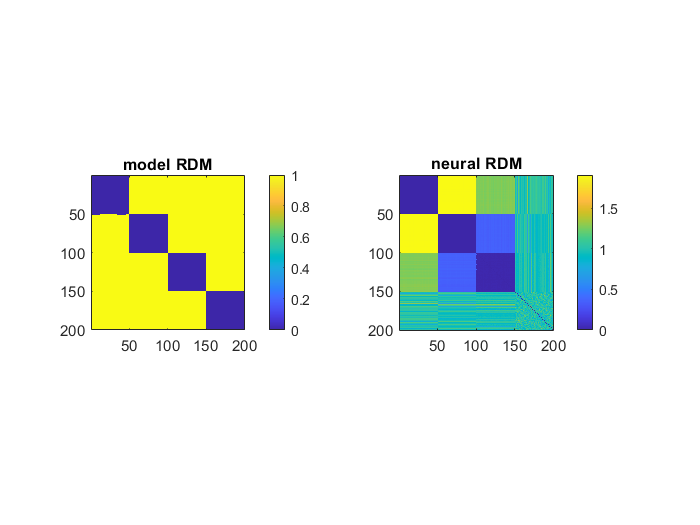
\includegraphics[width=\maxwidth{78.03311590566985em}]{figure_1.png}
\end{center}


\begin{par}
\begin{flushleft}
However, If we need to fit a large number of models and don't really need detailed statistics from each model, we can use the \href{https://www.mathworks.com/help/stats/regress.html}{`regress`} function to trade comprehensiveness for speed. 
\end{flushleft}
\end{par}

\begin{matlabcode}
% define outcome variable
y = data_2014.LE;
% define predictor variables
X = nan(length(y), 4); %%% initialize 3 columns
X(:, 1) = 1; %%% constant term is NOT automatically put into the model!
X(:, 2) = double(data_2014.Status=="Developing"); %%% manually code the categorical variable
X(:, 3) = data_2014.("Total expenditure") - mean(data_2014.("Total expenditure"), "omitmissing");
X(:, 4) = X(:, 2) .* X(:, 3); %%% interaction term
[b, bint, r, rint, stats] = regress(y, X);
b
\end{matlabcode}
\begin{matlaboutput}
b = 4x1    
   81.1316
  -11.2652
    0.0032
    0.7351

\end{matlaboutput}
\begin{matlabcode}
m3.Coefficients
\end{matlabcode}
\begin{matlabtableoutput}
{
\begin{tabular} {|c|c|c|c|c|}\hline
\mlcell{ } & \mlcell{Estimate} & \mlcell{SE} & \mlcell{tStat} & \mlcell{pValue} \\ \hline
\mlcell{1 (Intercept)} & \mlcell{81.1316} & \mlcell{1.4382} & \mlcell{56.4102} & \mlcell{0} \\ \hline
\mlcell{2 Status\_rev\_Developing} & \mlcell{-11.2652} & \mlcell{1.5557} & \mlcell{-7.2414} & \mlcell{0} \\ \hline
\mlcell{3 TE\_mc} & \mlcell{0.0032} & \mlcell{0.3812} & \mlcell{0.0085} & \mlcell{0.9932} \\ \hline
\mlcell{4 Status\_rev\_Developing:TE\_mc} & \mlcell{0.7351} & \mlcell{0.4512} & \mlcell{1.6292} & \mlcell{0.1050} \\ 
\hline
\end{tabular}
}
\end{matlabtableoutput}
\begin{matlabcode}
all(m3.Coefficients.Estimate == b)
\end{matlabcode}
\begin{matlaboutput}
ans = 
   1

\end{matlaboutput}

\begin{par}
\begin{flushleft}
Ta-da! As we can see the regression coefficients we obtained using `regress` are exactly the same as what we had from `fitlm` earlier, though we no longer have the nice-looking table filled with stats. However, the (very crude) test below shows that `regress` is indeed a lot faster than `fitlm`.
\end{flushleft}
\end{par}


\begin{matlabcode}
tic
for i=1:500
    y = data_2014.LE;
    % define predictor variables
    X = nan(length(y), 4); %%% initialize 3 columns
    X(:, 1) = 1; %%% constant term is NOT automatically put into the model!
    X(:, 2) = double(data_2014.Status=="Developing"); %%% manually code the categorical variable
    X(:, 3) = data_2014.("Total expenditure") - mean(data_2014.("Total expenditure"), "omitmissing");
    X(:, 4) = X(:, 2) .* X(:, 3); %%% interaction term
    [b, bint, r, rint, stats] = regress(y, X);
end
toc
\end{matlabcode}
\begin{matlaboutput}
Elapsed time is 0.201044 seconds.
\end{matlaboutput}
\begin{matlabcode}
tic
for i=1:500
    m = fitlm(data_2014, "LE ~ TE_mc * Status_rev");
end
toc
\end{matlabcode}
\begin{matlaboutput}
Elapsed time is 5.250400 seconds.
\end{matlaboutput}

\label{H_02A678E6}
\matlabheading{4. Conclusion}

\begin{par}
\begin{flushleft}
We've made it to the end of MATLAB basics and regression (yay!), though this is just the tip of the iceberge of regression models out in the wild world, such as regularized regression, nonlinear regression, and mixed-effects regression. Feel free to check out how they are can be implemented in MATLAB \href{https://www.mathworks.com/help/stats/introduction-to-parametric-regression-analysis.html}{here}. 
\end{flushleft}
\end{par}

\begin{par}
\begin{flushleft}
Enjoying MATLAB-ing!
\end{flushleft}
\end{par}

\end{document}
